\documentclass[12pt,a4paper]{article}

\usepackage[T1,T2A]{fontenc}
\usepackage[utf8]{inputenc}
\usepackage[english,russian]{babel}
\usepackage{microtype}
\usepackage{csquotes}
\usepackage{amsmath}
\usepackage{amsthm}
\usepackage{amssymb}
\usepackage{mathtext}
\usepackage{physics}
\usepackage{newfloat}
\usepackage{caption}
\usepackage{indentfirst}
\usepackage{titlesec,titletoc}
\usepackage{geometry}
\usepackage{hyperref}
\usepackage{mdframed}
\usepackage[inline]{enumitem}
\usepackage{graphicx}
\usepackage{subfig}
\usepackage[titletoc,toc]{appendix}

\DeclareGraphicsExtensions{.pdf,.png,.jpg,.PNG}
\graphicspath{{./img/}}
\captionsetup[figure]{justification=centering}
\renewcommand{\thesubfigure}{\asbuk{subfigure}}
\DeclareCaptionLabelSeparator{dotseparator}{. }
\captionsetup{labelsep=dotseparator}
\geometry{left=1cm,right=1cm,top=2cm,bottom=2cm}
\makeatletter\appto{\appendices}{\def\Hy@chapapp{Appendix}}\makeatother
\renewcommand{\appendixtocname}{Приложения}
\renewcommand{\appendixpagename}{Приложения}

\DeclareMathOperator{\Rot}{\mathbf{rot}}
\DeclareMathOperator{\Grad}{\mathbf{grad}}
\DeclareMathOperator{\Div}{\mathbf{div}}
\DeclareMathOperator{\D}{D}
\newcommand{\V}[1]{\mathbf{#1}}
\newcommand{\Op}[1]{\hat{\V{#1}}}


\title{Термодинамика сферических резонаторов}
\author{Василевский А.В.}

\begin{document}

    \maketitle
    \tableofcontents

    \section{Термодинамика сферических резонаторов}

    %
    %
    %
    %%%%%%%%%%%%%%%%%%%%%%%%%%%%%%%%%%%%%%%%%%%%%%%%%%%%%%%%%%%%%%%%%%%%%%%
    %                           SUBSUBSECTION                             %
    %%%%%%%%%%%%%%%%%%%%%%%%%%%%%%%%%%%%%%%%%%%%%%%%%%%%%%%%%%%%%%%%%%%%%%%
    %
    %
    %

    \subsection*{Введение}

        Целью данной работы является построение термодинамики электромагнитного поля в сферическом резонаторе.

        Нам уже известен возможный спектр мод электромагнитного поля. Дальнейшей задачей становится получение спектральной плотности запасенной в резонаторе энергии подобно планковскому закону излучения абсолютно черного тела.

    %
    %
    %
    %%%%%%%%%%%%%%%%%%%%%%%%%%%%%%%%%%%%%%%%%%%%%%%%%%%%%%%%%%%%%%%%%%%%%%%
    %                           SUBSUBSECTION                             %
    %%%%%%%%%%%%%%%%%%%%%%%%%%%%%%%%%%%%%%%%%%%%%%%%%%%%%%%%%%%%%%%%%%%%%%%
    %
    %
    %

    \subsection{Спектральная плотность энергии. Формула Планка}

        К построению кривой спектральной плотности энергии $u(\omega)$ будем подходить методами статистики через количество фотонов с данной энергией в единице объема пространства.

        Фотоны подчиняются статистике Бозе-Эйнштейна, потому для среднего числа частиц с данной энергией $\varepsilon = \hbar \omega$ справедливо
        %
        \begin{equation}
            n(\varepsilon) = \frac{1}{\exp(\flatfrac{\varepsilon}{kT}) - 1} .
        \end{equation}
        %
        Спектральная плотность энергии может быть выражена как
        %
        \begin{equation}\label{eq:psd}
            u(\omega) \dd{\omega} = \hbar\omega\ n(\hbar\omega) \dd{N(\omega)} ,
        \end{equation}
        %
        где $N(\varepsilon)$~--- число мод электромагнитного поля в единице объема пространства с частотами в бесконечно малой окрестности $\omega$. Таким образом, для получения $u(\omega)$ необходимо лишь знать вид $\dv*{N}{\omega}$.

        Можно показать \cite{sivuhin_opt}, что число стоячих волн с частотами $[\omega,\omega+\dd{\omega}]$ в единице объема трехмерного пространства асимптотически ($\omega \to \infty$) распределено в соответствии с законом
        %
        \begin{equation}\label{eq:dN_of_eps_cont}
            \dd{N(\omega)} = \frac{\omega^2 \dd{\omega}}{\pi^2 v^3} .
        \end{equation}
        %
        Как и ранее, $v$ здесь обозначает скорость света в среде. При подстановке \autoref{eq:dN_of_eps_cont} в \autoref{eq:psd} спектральная плотность энергии $u(\omega)$ приобретает известный вид:
        %
        \begin{equation}
            u(\omega) = \frac{
                    \flatfrac{\omega^2 \hbar\omega}{\pi^2 v^3}
            }{\exp(\flatfrac{\hbar\omega}{kT}) - 1} .
        \end{equation}
        %
        Это знаменитая формула Планка, полученная им для излучения абсолютно черного тела.

    %
    %
    %
    %%%%%%%%%%%%%%%%%%%%%%%%%%%%%%%%%%%%%%%%%%%%%%%%%%%%%%%%%%%%%%%%%%%%%%%
    %                           SUBSECTION                                %
    %%%%%%%%%%%%%%%%%%%%%%%%%%%%%%%%%%%%%%%%%%%%%%%%%%%%%%%%%%%%%%%%%%%%%%%
    %
    %
    %

    \subsection{Построение кривой спектральной плотности энергии}

        Перейдем к непосредственному построению спектральной плотности энергии поля в резонаторе.

        Ранее было показано, что собственные частоты резонатора $\omega_n$ определяется нулями радиальных частей сферических мод. Известно, что радиальная часть моды зависит только от $l$ и не зависит от $m \in \qty[-l,l]$. Следовательно, $l$-я мода является $2l + 1$-вырожденной по энергии.

        Будем обозначать собственные частоты, полученные из граничных условий для $p$-поляризованной $l$-й моды, как $\omega^{lp}_n$, т.е. снабдим существующий набор $\omega_n$ дополнительными индексами. Будем также для удобства предполагать, что $\omega_n$ упорядочены по $n$: всегда выполняется $\omega_{n-1} \le \omega_n$. В таких обозначениях некоторой данной $\omega^{lp}_n$ соответствует $2l + 1$.

        Дальнейшая наша задача сводится к следующему. Необходимо показать, что и в случае сферического резонатора наблюдается асимптотическое поведение $\dv*{N}{\omega} \sim \omega^2$ при больших $\omega$. Для этого необходимо посчитать $\dv*{N}{\omega} \approx \flatfrac{\Delta N}{\Delta \omega}$ по существующему спектру мод, т.е. фактически произвести свертку функции дискретного аргумента $N(\omega^{lp}_n) = 2l + 1$ с окном $\Delta \omega$.

        Изобразим функцию $N(\omega_n)$ (\autoref{fig:n}). Каждая \enquote{строчка} функции соответствует аргументам $\omega^{lp}_i$ для обеих значений $p$ и фиксированного значения $l$. Численно $\omega^{lp}_i$ являются нулями радиальных функций. С увеличением $l$ независимо от поляризации увеличивается также и положение самого левого нуля радиальной функции. Нули радиальных функций обеих поляризаций находятся близко друг к другу. Асимптотически при $i \to \infty$ расстояние между соседними нулями каждой из радиальных функций стремится к $\pi$.
        %
        \begin{figure}[h]
            \centering
            %
            \subfloat[][]{%
                \label{fig:n_all}%
                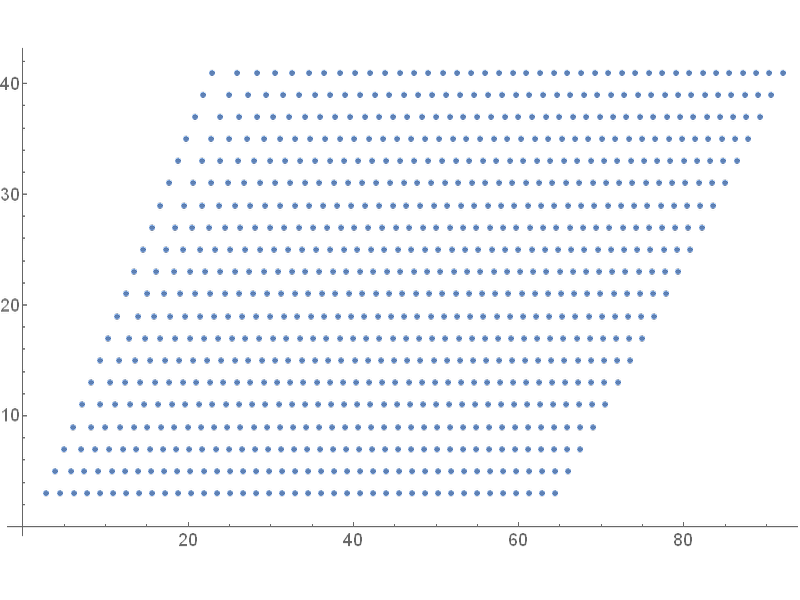
\includegraphics[width=0.45\textwidth]{n}}%
            \hspace{8pt}%
            %
            \subfloat[][]{%
                \label{fig:n_full}%
                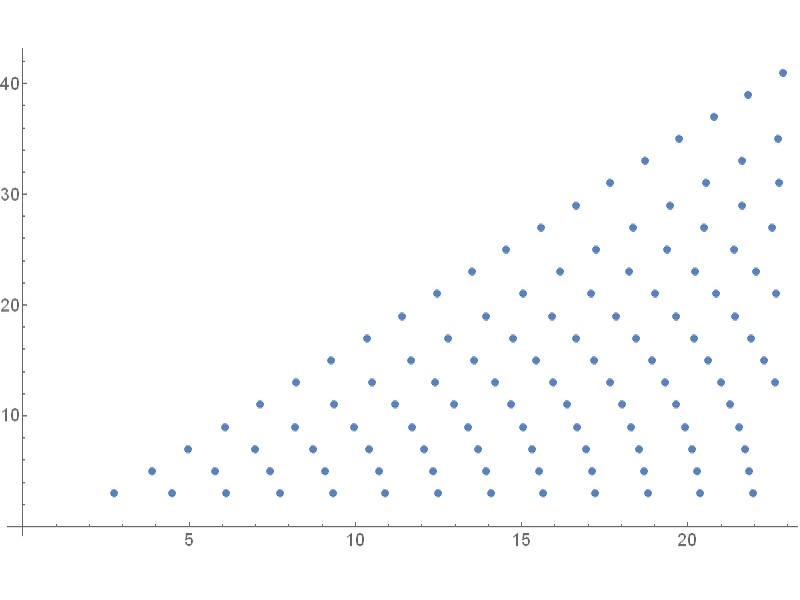
\includegraphics[width=0.45\textwidth]{n_full}}%
            \hspace{8pt}%
            %
            \caption[]{Функция $N(\omega_n)$ (аргумент в относительных единицах). Параметр $l_{max} = 300$. На \subref{fig:n_full} увеличена область $\omega < \Omega$. %
            } %
            \label{fig:n}%
        \end{figure}

        Описанная картина говорит о следующем. Пусть мы имеем некоторый рассчитанный конечный набор $\omega^{lp}_n$, $n = 1, 2, \dots, n_{max}$, полученный из $2 * (l_{max} - l_{min})$ различных базовых мод (двойка соответствует числу возможных поляризаций). В области $0 < \omega \le \Omega = \min_p{\omega^{l_{max}p}_{i_{min}}}$, где $i_{min}$~--- индекс самого левого нуля $l_{max}$-й радиальной функции $p$-й поляризации, имеется полная информация о функции $N(\omega_n)$. Иными словами, в этой области она построена по всем своим возможным аргументам. В области $\omega > \Omega$ отсечены значения функции $N(\omega^{lp}_n)$ с $l > l_{max}$, потому она не пригодна для дальнейшего рассмотрения. Под $l_{min}$ здесь понимается минимальное физически возможное значение $l$. Ранее было показано, что $l_{min} = 1$.

        На \autoref{fig:dndx} изображена функция $\flatfrac{\Delta N}{\Delta \omega}$ в области $\omega < \Omega - \Delta\omega / 2$. Видно, что результат свертки визуально похож на квадратичную функцию. Это подтверждает также и изображенная поверх множества точек непрерывная функция. Коэффициенты функции были получены методом минимизации функционала квадратичной нормы отклонения непрерывной функции от дискретных точек $\flatfrac{\Delta N}{\Delta \omega}$. По \autoref{fig:dndx}\subref{fig:dndx_mag} видно, что дискретные точки ложатся на непрерывную кривую уже при совсем небольших значениях $\omega_n$.
        %
        \begin{figure}[h]
            \centering
            %
            \subfloat[][]{%
                \label{fig:dndx_all}%
                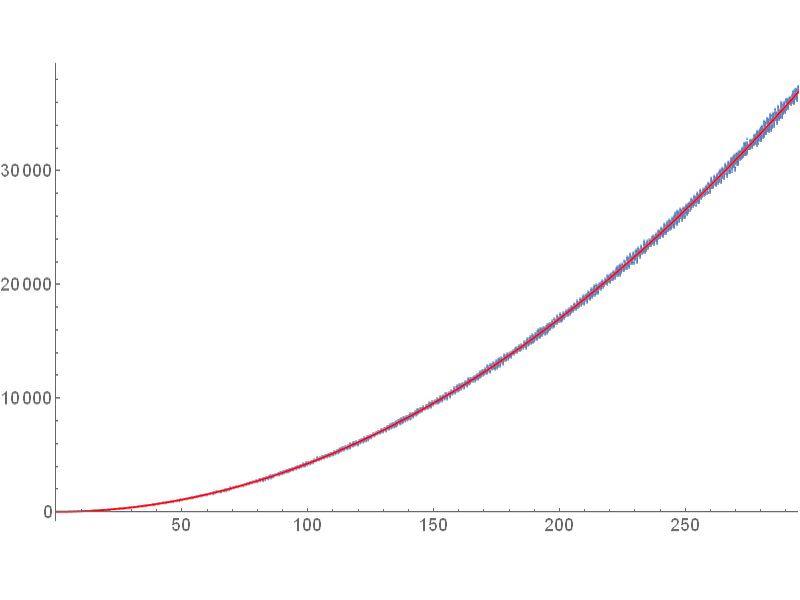
\includegraphics[width=0.45\textwidth]{dndx}}%
            \hspace{8pt}%
            %
            \subfloat[][]{%
                \label{fig:dndx_mag}%
                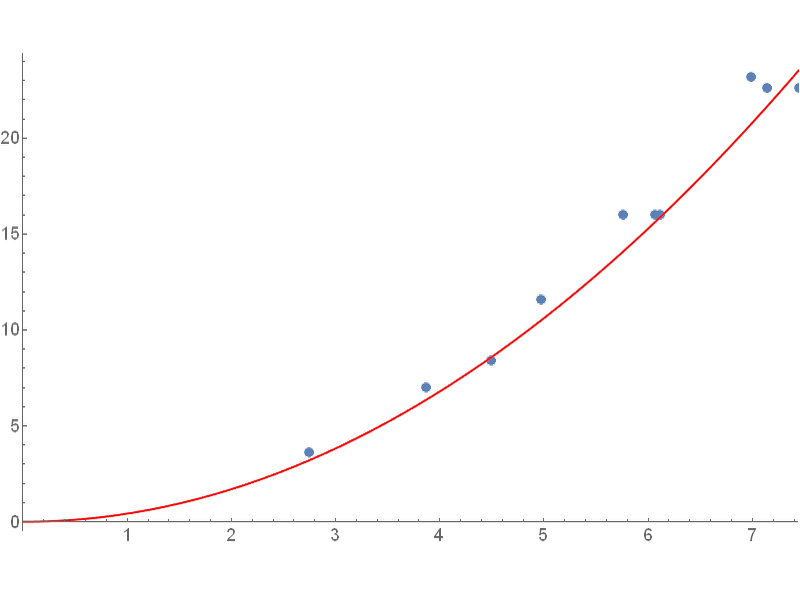
\includegraphics[width=0.45\textwidth]{dndx_mag}}%
            \hspace{8pt}%
            %
            \caption[]{Функция $\flatfrac{\Delta N}{\Delta \omega}$ (аргумент в относительных единицах), дискретная и непрерывная. Параметр $l_{max} = 300$. Размер окна~--- 5 относительных единиц. На \subref{fig:dndx_mag} увеличена область вблизи нуля. %
            } %
            \label{fig:dndx}%
        \end{figure}

        Более детально вопрос непосредственного получения $\flatfrac{\Delta N}{\Delta \omega}$ описан в \autoref{sec:getting_plank_formula}.

        Итак, мы показали, что асимптотически $\flatfrac{\Delta N}{\Delta \omega} \sim \omega^2$, причем данное соответствие имеет место уже при совсем небольших значениях $\omega$. Это, в свою очередь, доказывает справедливость формулы Планка и в случае сферических резонаторов. На \autoref{fig:plank} изображена кривая спектральной плотности энергии по дискретным данным с наложенной на нее классической непрерывной кривой. Как и ожидалось, кривые совпадают.
        %
        \begin{figure}[h]
            \centering
            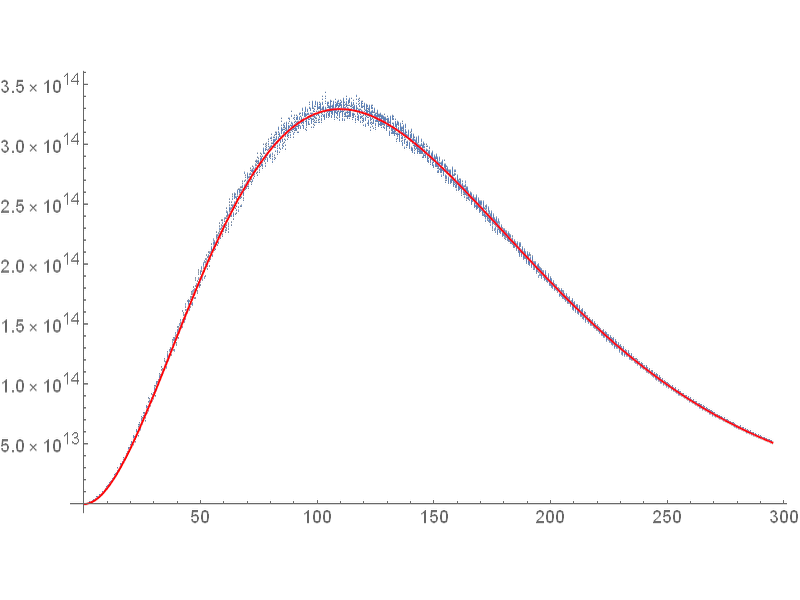
\includegraphics[width=0.5\textwidth]{plank}
            \caption[]{Планковская кривая, практическая (дискретная, построенная на данных \autoref{fig:dndx}) и теоретическая (непрерывная). Единицы относительные.}
            \label{fig:plank}
        \end{figure}

    %
    %
    %
    %%%%%%%%%%%%%%%%%%%%%%%%%%%%%%%%%%%%%%%%%%%%%%%%%%%%%%%%%%%%%%%%%%%%%%%
    %                          APPENDIX                                   %
    %%%%%%%%%%%%%%%%%%%%%%%%%%%%%%%%%%%%%%%%%%%%%%%%%%%%%%%%%%%%%%%%%%%%%%%
    %
    %
    %

    \begin{subappendices}

    %
    %
    %
    %%%%%%%%%%%%%%%%%%%%%%%%%%%%%%%%%%%%%%%%%%%%%%%%%%%%%%%%%%%%%%%%%%%%%%%
    %                           SUBSECTION                                %
    %%%%%%%%%%%%%%%%%%%%%%%%%%%%%%%%%%%%%%%%%%%%%%%%%%%%%%%%%%%%%%%%%%%%%%%
    %
    %
    %

    \subsection{Вычисление распределения мод по частотам\label{sec:getting_plank_formula}}

        В данной секции мы подробно рассмотрим вопрос получения асимптотической функции $\flatfrac{\Delta N}{\Delta \omega}$.

        Фактически данная функция является сверткой функции $N(\omega_n)$ с прямоугольным окном ширины $\Delta \omega$. Действительно, $\Delta N$ носит смысл количества мод в некоторой малой окрестности $\omega_n$, потому может быть вычислена как сумма значений функции $N(\omega_n)$ (смысл которой, напомним, количество мод, имеющих собственную частоту точно $\omega_n$) в пределах некоторого окна $\Delta \omega$. Запишем это математически:
        %
        \begin{equation}
            \Delta N(\omega) = \sum\limits_{
                \qty|\omega - \omega_n| < \Delta\omega/2
            } N(\omega_n) = \qty(W_{\Delta\omega} \vdot N)(\omega) .
        \end{equation}
        %
        Здесь $W_{\Delta\omega}$~--- прямоугольная оконная функция, $\Delta\omega$ носит характер ширины окна, операция свертки обозначена через $(f \vdot g)(x)$. Нам остается лишь только поделить $\Delta N$ на ширину окна $\Delta\omega$, чтобы получить окончательно $\flatfrac{\Delta N}{\Delta \omega}$. Следует отметить, что при таком определении $\Delta N(\omega)$ не важно, является ли аргумент $\omega$ одной из собственных частот $\omega_n$. В то время как расстояние $\omega_{n+1} - \omega_n$ не является фиксированным, мы можем получить функцию $\Delta N(\omega)$ с фиксированным шагом по аргументу или же в промежуточных точках \enquote{$\omega_{n+1/2}$}.

        До сих пор мы говорили, что последовательность $\omega_n$ нам известна. На самом деле ее получение вызывает некоторые трудности. Каждая из собственных частот резонатора $\omega^{lp}_n$ получается из граничных условий на $l$-ю моду $p$-й поляризации. Граничные условия в конечном счете требуют
        %
        \begin{equation}\begin{aligned}
            S_l(\sqrt\lambda r_\text{шара}) &= 0
                \quad \text{для $\mathrm{II}$ поляризации} , \\
            S'_l(\sqrt\lambda r_\text{шара}) &= 0
                \quad \text{для $\mathrm{I}$ поляризации},
        \end{aligned}\end{equation}
        %
        где $S_l$~--- функция Риккати-Бесселя, а $S'_l$~--- ее производная по аргументу, $\lambda = \varepsilon \flatfrac{\omega^2}{c^2}$. Если обозначить аргумент $\sqrt\lambda r_\text{шара} \sim \omega$ за $x$, то уравнения на собственные частоты резонатора перепишутся в виде
        %
        \begin{equation}\begin{aligned}
            S_l(x) &= 0, \\
            S'_l(x) &= 0.
        \end{aligned}\end{equation}
        %
        Приступим к их решению.

        Уравнения выше записаны в симметричной форме, однако учитывая то, что $S_l(x) = x j_l(x) = \sqrt{\flatfrac{\pi x}{2}} J_{l+1/2}(x)$, где $J_{l+1/2}(x)$~--- функция Бесселя первого рода полуцелого порядка $l + 1/2$, первое уравнение можно упростить до
        %
        \begin{equation}
            J_{l+1/2}(x) = 0 ,
        \end{equation}
        %
        для решения которого разработаны эффективные численные процедуры поиска корней (см. напр. \cite{handbook_of_math_functions}).

        Снова представляя $S_l(x)$ через $J_{l+1/2}(x)$, запишем эквивалентное второму уравнение
        %
        \begin{equation}
            \dv{x}(\sqrt{x} J_{l+1/2}(x)) = 0 .
        \end{equation}
        %
        Для его решения нет специальных численных схем, поэтому мы будем пытаться свести процедуру решения к известным схемам. В частности, известна процедура поиска нулей функции $J'_{l+1/2}(x)$. Уравнение выше можно рассматривать как уравнение на экстремумы функции, стоящей под знаком производной. Очевидно, что экстремумы $J_{l+1/2}(x)$ будут находиться между ее нулями. Положение экстремумов изменится не сильно, кроме того, они сместятся в одном и том же направлении, если функцию $J_{l+1/2}(x)$ умножить на монотонно возрастающую функцию $\sqrt{x}$. Это, в свою очередь, означает, что нули $J'_{l+1/2}(x)$ являются хорошим приближением для нулей $(\sqrt{x} J_{l+1/2}(x))'$. Можно построить процедуру поиска нулей целевой функции через уточнение нулей $J'_{l+1/2}(x)$.

        Можно пойти еще дальше. Несложно заметить, что корни как первого, так и второго уравнения подчиняются следующим закономерностям. Если обозначить корни первого или второго уравнения за $x^n_l$, $x^n_l < x^{n+1}_l$, то можно показать, что для одного и того же $n$ выполняется
        %
        \begin{equation}
            \frac{\pi}{4} < x^n_{l + 1} - x^n_l < \frac{\pi}{2} ,
        \end{equation}
        %
        причем приближение к левой границе осуществляется с увеличением $l$, а к правой~--- с ростом $n$. Участок $\qty[x^n_l + \flatfrac{\pi}{4}, x^n_l + \flatfrac{\pi}{2}]$ является участком монотонности целевой функции, так что на нем хорошо применимы традиционные численные методы поиска нуля, например метод Ньютона.

        Исходя из этих соображений, мы можем построить рекуррентную процедуру численного поиска корней обоих уравнений. Зададимся некоторыми значениями $l_{min}$, $l_{max}$ и $n_{max}$. Тогда для первого уравнения процедура будет сводиться к следующему:
        %
        \begin{enumerate}[nosep]
            \item ищутся корни $x^n_{l_{min}}$, $n = 1, 2, \dots, n_{max}$ функции $J_{l+1/2}(x)$ известными специальными методами;
            \item поиск корней $x^n_{l+1}$, $n = 1, 2, \dots, n_{max}$ организуется в интервале $\qty[x^n_l + \flatfrac{\pi}{4}, x^n_l + \flatfrac{\pi}{2}]$ обычными численными методами, пока не будут найдены корни для всех $l \le l_{max}$.
        \end{enumerate}
        %
        Для второго уравнения добавится лишь один дополнительный шаг:
        %
        \begin{enumerate}[nosep]
            \item за начальное приближение $x^n_{l_{min}}$, $n = 1, 2, \dots, n_{max}$ выбираются нули $J'_{l+1/2}(x)$,
            \item они уточняются для целевой функции в интервале $\qty[x^n_{l_{min}} + \flatfrac{\pi}{4}, x^n_{l_{min}} + \flatfrac{\pi}{2}]$ обычными численными методами,
            \item поиск корней $x^{l+1}_n$, $n = 1, 2, \dots, n_{max}$ организуется в интервале $\qty[x^n_l + \flatfrac{\pi}{4}, x^n_l + \flatfrac{\pi}{2}]$ как в предыдущем случае.
        \end{enumerate}

        Поговорим о сам\'{о}й функции $N(\omega_n)$. Мы знаем, что $l$-я мода $2l + 1$-кратно вырождена по энергии. Это равносильно утверждению, что одной собственной энергии $\omega^{lp}_n$ соответствует $2l + 1$ мода. Поэтому значение функции $N(\omega^{lp}_n) = 2l + 1$. Функция $N(\omega_n)$ изображена на \autoref{fig:n}.

        Ранее отмечалось, что в области $0 < \omega < \Omega$, где $\Omega = \min_p{\omega^{l_{max}p}_{i_{min}}}$~--- первый нуль $l_{max}$-й радиальной функции одной из поляризаций, мы имеем полную информацию о распределении мод по частотам. Действительно, в области $\omega > \Omega$ отсутствуют нули функций б\'{о}льших порядков, поэтому она не содержит полной информации и непригодна для дальнейшего исследования. Подробно рассмотрим первую область.

        Найдем функцию $(\flatfrac{\Delta N}{\Delta \omega})(\omega)$ описанным выше способом, пока выбирая в качестве $\omega$ значения собственных частот резонатора $\omega_n$. Мы обнаружим, что в области $\Delta\omega / 2 < \omega < \Omega - \Delta\omega / 2$ (поправка на полуширину окна вводится для устранения \enquote{краевых эффектов} свертки) данная функция хорошо аппроксимируется квадратичной функцией (\autoref{fig:dndx}), причем качество аппроксимации увеличивается с увеличением доступного $l_{max}$: коэффициент корреляции Пирсона стремится к единице\footnotemark{}. Это говорит об асимптотическом характере зависимости $(\Delta N)(\omega) \sim \omega^2$. В области вблизи нуля (\autoref{fig:dndx}\subref{fig:dndx_mag}) все же не наблюдается значительных отклонений $\flatfrac{\Delta N}{\Delta \omega}$ от аппроксимирующей квадратичной функции, потому можно говорить, что с большой точностью $(\Delta N)(\omega) \sim \omega^2$ верно и для близких к нулю собственных частот.

        \footnotetext{
            Конкретные цифры в работе не приводятся. Они зависят от выбранной методики проведения расчетов, их точности, от вида функционала ошибки в аппроксимационной схеме и т.д. На наш взгляд достаточно и того, что визуально зависимости накладываются друг на друга, причем коэффициент при $\omega^2$ с некоторой точностью совпадает с теоретическим. Отметим лишь, что уже при $l_\text{max} = 50$ и ширине окна $\Delta \omega \sim \Delta x = 10$ ошибка в определении коэффициента не превышала $0.6\%$ при коэффициенте корреляции около $0.9998$. При увеличении $l_\text{max}$ точность вычислений только возрастала.
        }

        Поскольку $\flatfrac{\Delta N}{\Delta \omega}$ можно с высокой точностью описывать квадратичным законом в широких пределах изменения $\omega$, спектральная плотность энергии будет очень хорошо ложиться на планковскую кривую даже в области близких к нулю частот. Запишем выражение для $u(\omega)$ в единицах переменной $x$:
        %
        \begin{equation}\begin{aligned}
            u(x)
                &= \frac{1}{\pi^2 r_\text{шара}^3}
                    x n(x) \qty(\frac{\Delta N}{\Delta x})(x) \\
                &= \frac{\flatfrac{x^3}{\pi^2 r_\text{шара}^3}}{
                        \exp\qty(\frac{\hbar v x}{kT r_\text{шара}}) - 1
                    } .
        \end{aligned}\end{equation}
        %
        Кривая $u(x)$ для некоторого значения $r_\text{шара}$ изображена на \autoref{fig:plank}. Необходимо помнить о том, что $u(\omega)$~--- спектральная плотность энергии \textit{на единицу объема}, в то время как найденная выше функция $\flatfrac{\Delta N}{\Delta x}$ приходится \textit{на весь объем резонатора}. Поэтому перед подстановкой в данную формулу $\flatfrac{\Delta N}{\Delta x}$ следует поделить на объем резонатора, т.е. на величину $V_\text{шара} = \flatfrac{4}{3} \pi r_\text{шара}^3$.

    \end{subappendices}

    %
    %
    %
    %%%%%%%%%%%%%%%%%%%%%%%%%%%%%%%%%%%%%%%%%%%%%%%%%%%%%%%%%%%%%%%%%%%%%%%
    %                        BIBLIOGRAPHY                                 %
    %%%%%%%%%%%%%%%%%%%%%%%%%%%%%%%%%%%%%%%%%%%%%%%%%%%%%%%%%%%%%%%%%%%%%%%
    %
    %
    %

    \nocite{*}
    \bibliographystyle{../../lib/doc/bib/utf8gost705s}
    \bibliography{../../lib/doc/bib/physics,../../lib/doc/bib/math,math,physics}

\end{document}
